% !TeX root = proposal.tex
\chapter{Proposed Work}\label{chapter:evaluation}

To further explore this trade-off between parsimony and accuracy and to answer the second research question in Chapter~\ref{chapter:intro}, I propose the following user study plan focusing on evaluating the user experience of the privacy-setting interface prototypes.

\section{Planned Experimental Setup}
Proposed user study will be a between-subject study. All the participants will be recruited through Amazon Mechanical Turk. During this user study, we will manipulate two different independent variables to compare several default/profile solutions. The first one is the extend of default/profile's conservatives. We consider the default settings that with all disabled by default as the most conservative profile; and the default settings with all enabled by default as the most open profile, the `smart default' and `smart profiles' are considered to be in the middle. The other independent variable is the different levels of complexity for the settings interface. Hence $4$x$2=8$ total experimental conditions (i.e., user interfaces) will be presented to the participants. The Dependent variable of our study will be the user experience of the system, including the satisfaction and trust to the company.

During the user study~\footnote{The user study url can be found here: http://yyhe.people.clemson.edu/uistudy/}, the users will be first be welcome with brief introduction of the experimental instructions (See Figure~\ref{fig:us1}), followed by a participant consent form (See Figure~\ref{fig:us2}).

\begin{figure}
	\centering
	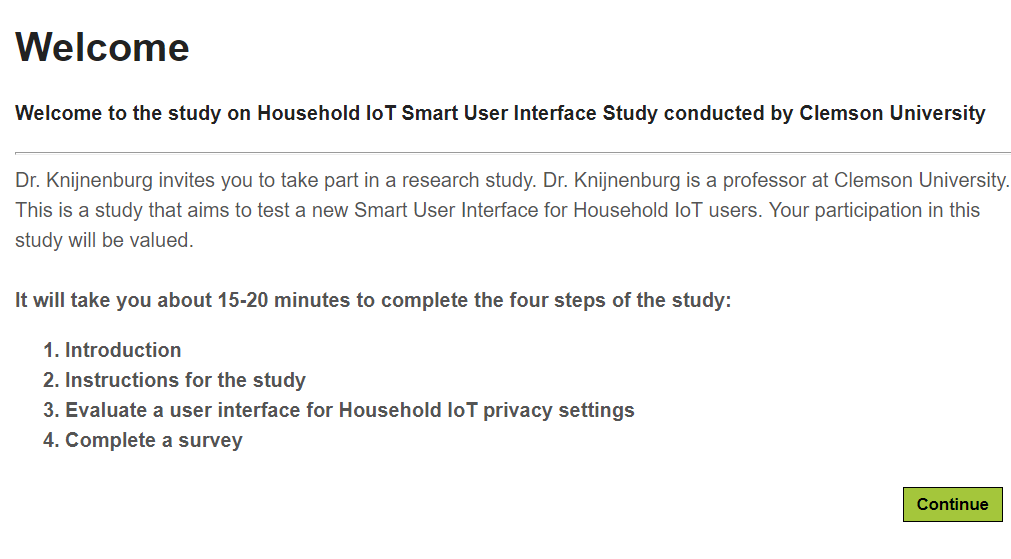
\includegraphics[width=0.48\textwidth]{figures/userstudy1.png}
	\caption{Experiment Landing Page}
	\label{fig:us1}
\end{figure}

\begin{figure}
	\centering
	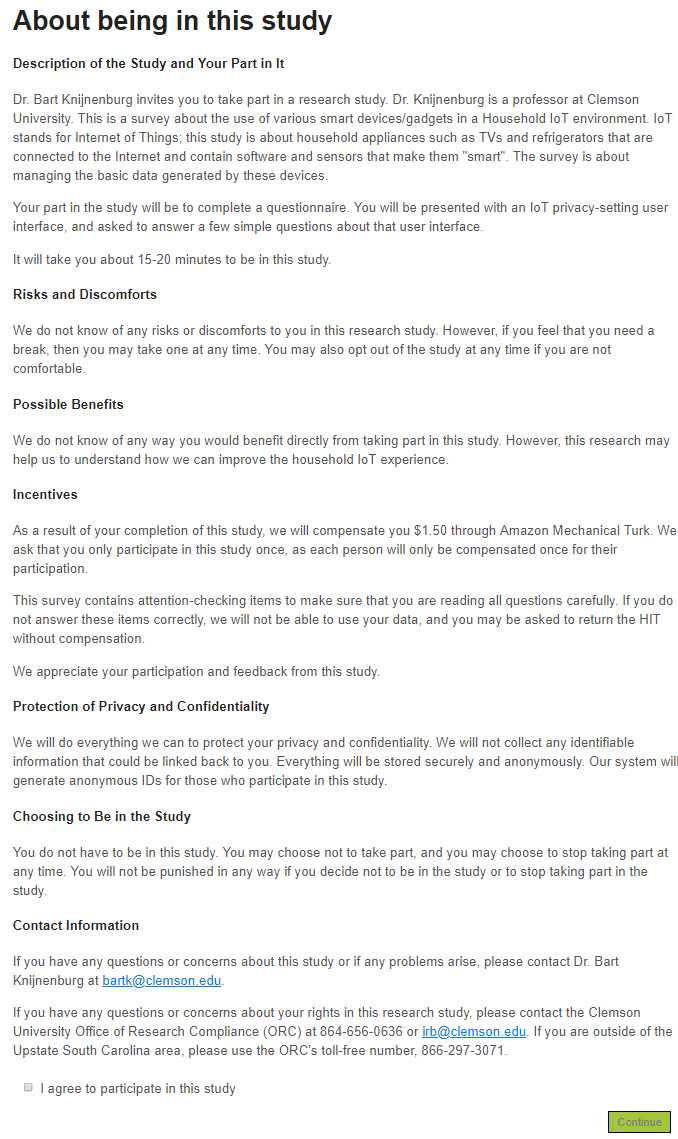
\includegraphics[width=0.48\textwidth]{figures/userstudy2.png}
	\caption{User Consent Form}
	\label{fig:us2}
\end{figure}

Then the participants will be introduced with the concept of the household IoT devices that appearing in this study, corresponding to the `Who' and `What' parameters of an IoT scenario. As shown in Figure~\ref{fig:us3}, the introduction contains both figures, text, and audio information. After the introduction, the participant will be given an example scenario to further understand the context of our study. Attention checks will also be given here to make sure the participants have paid attention to the explanations.
\begin{figure}
	\centering
	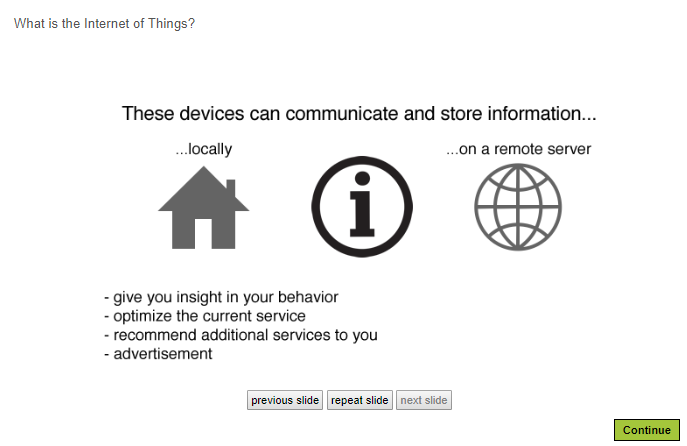
\includegraphics[width=0.48\textwidth]{figures/userstudy3.png}
	\caption{Introduction to Household IoT}
	\label{fig:us3}
\end{figure}

After above procedures, one out of the 8 user interfaces will be randomly chosen for each participants. Participants need to go through the whole interface to see if the preset privacy settings is suitable for them, and make necessary changes to accommodate their actual privacy demands. All these changes will be recorded to compared with the preset settings for further analysis purpose. A simple user interface condition with all settings turned off is shown in Figure~\ref{fig:ui1AllOff}.

\begin{figure}
	\centering
	\begin{subfigure}[t]{0.24\textwidth}
		\centering
		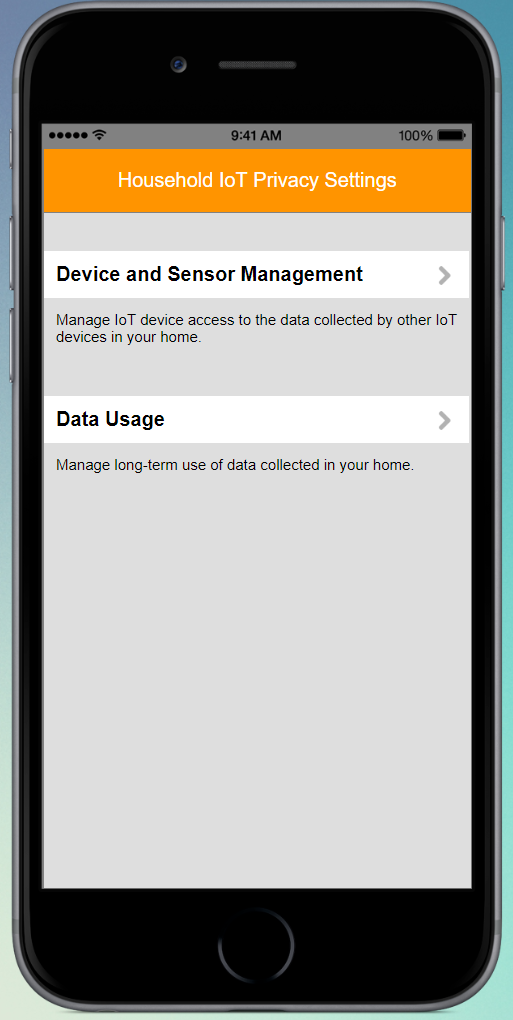
\includegraphics[height=2.8in]{figures/ui1allOff.png}
	\end{subfigure}%
	~
	\begin{subfigure}[t]{0.24\textwidth}
		\centering
		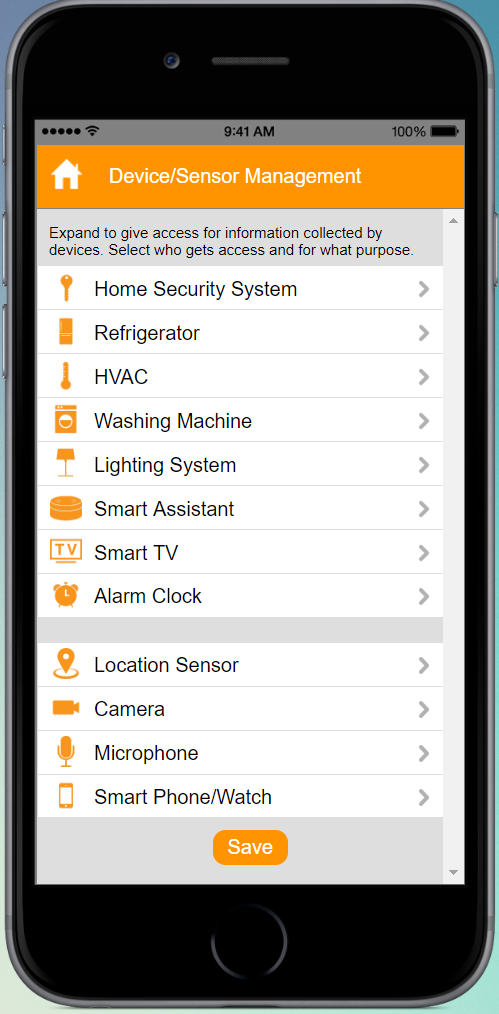
\includegraphics[height=2.8in]{figures/ui1allOff2.png}
	\end{subfigure}%
	~
	\begin{subfigure}[t]{0.24\textwidth}
		\centering
		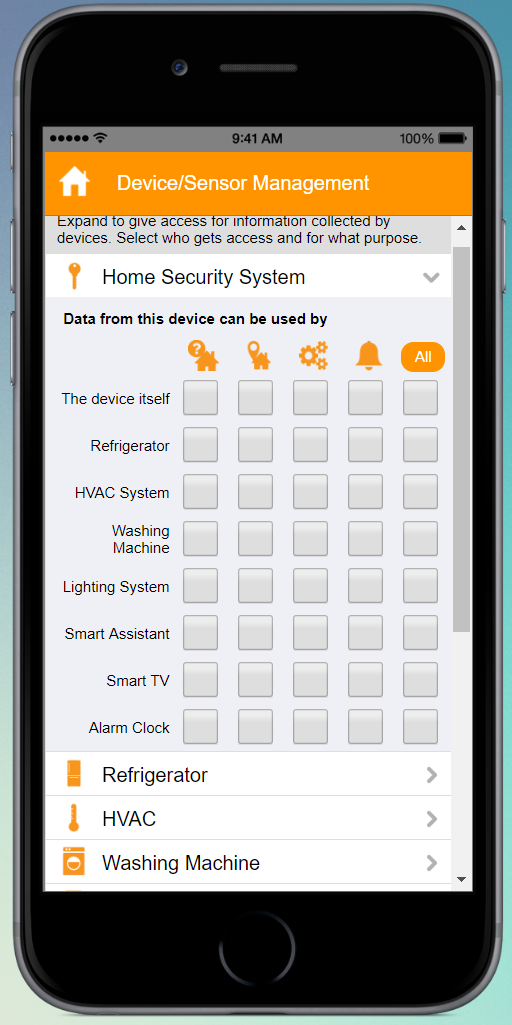
\includegraphics[height=2.8in]{figures/ui1allOff3.png}
	\end{subfigure}%
	~
	\begin{subfigure}[t]{0.24\textwidth}
		\centering
		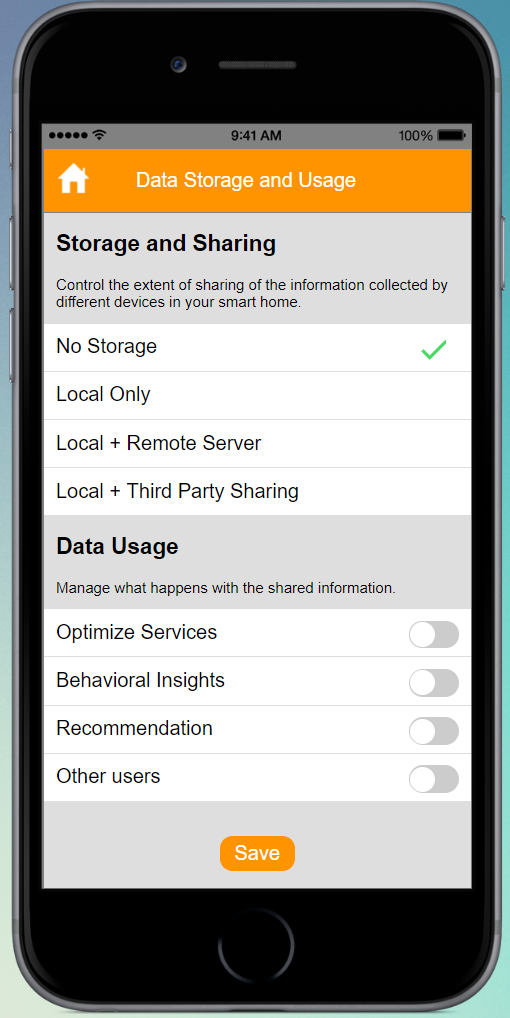
\includegraphics[height=2.8in]{figures/ui1allOff4.png}
	\end{subfigure}%
	\caption{Simple User-Interface condition with all settings turned off}
	\label{fig:ui1AllOff}
\end{figure}

Next, the participants will be give a survey containing questions about three different aspects: \textit{Subjective System Aspects} (Orange color), \textit{Personal Characteristics} (Blue color), and \textit{Situational Characteristics} (Green color), as shown in Figure~\ref{fig:uimodel}. All the items of the questionnaire are shown in Appendix.

%\begin{figure}
%	\centering
%	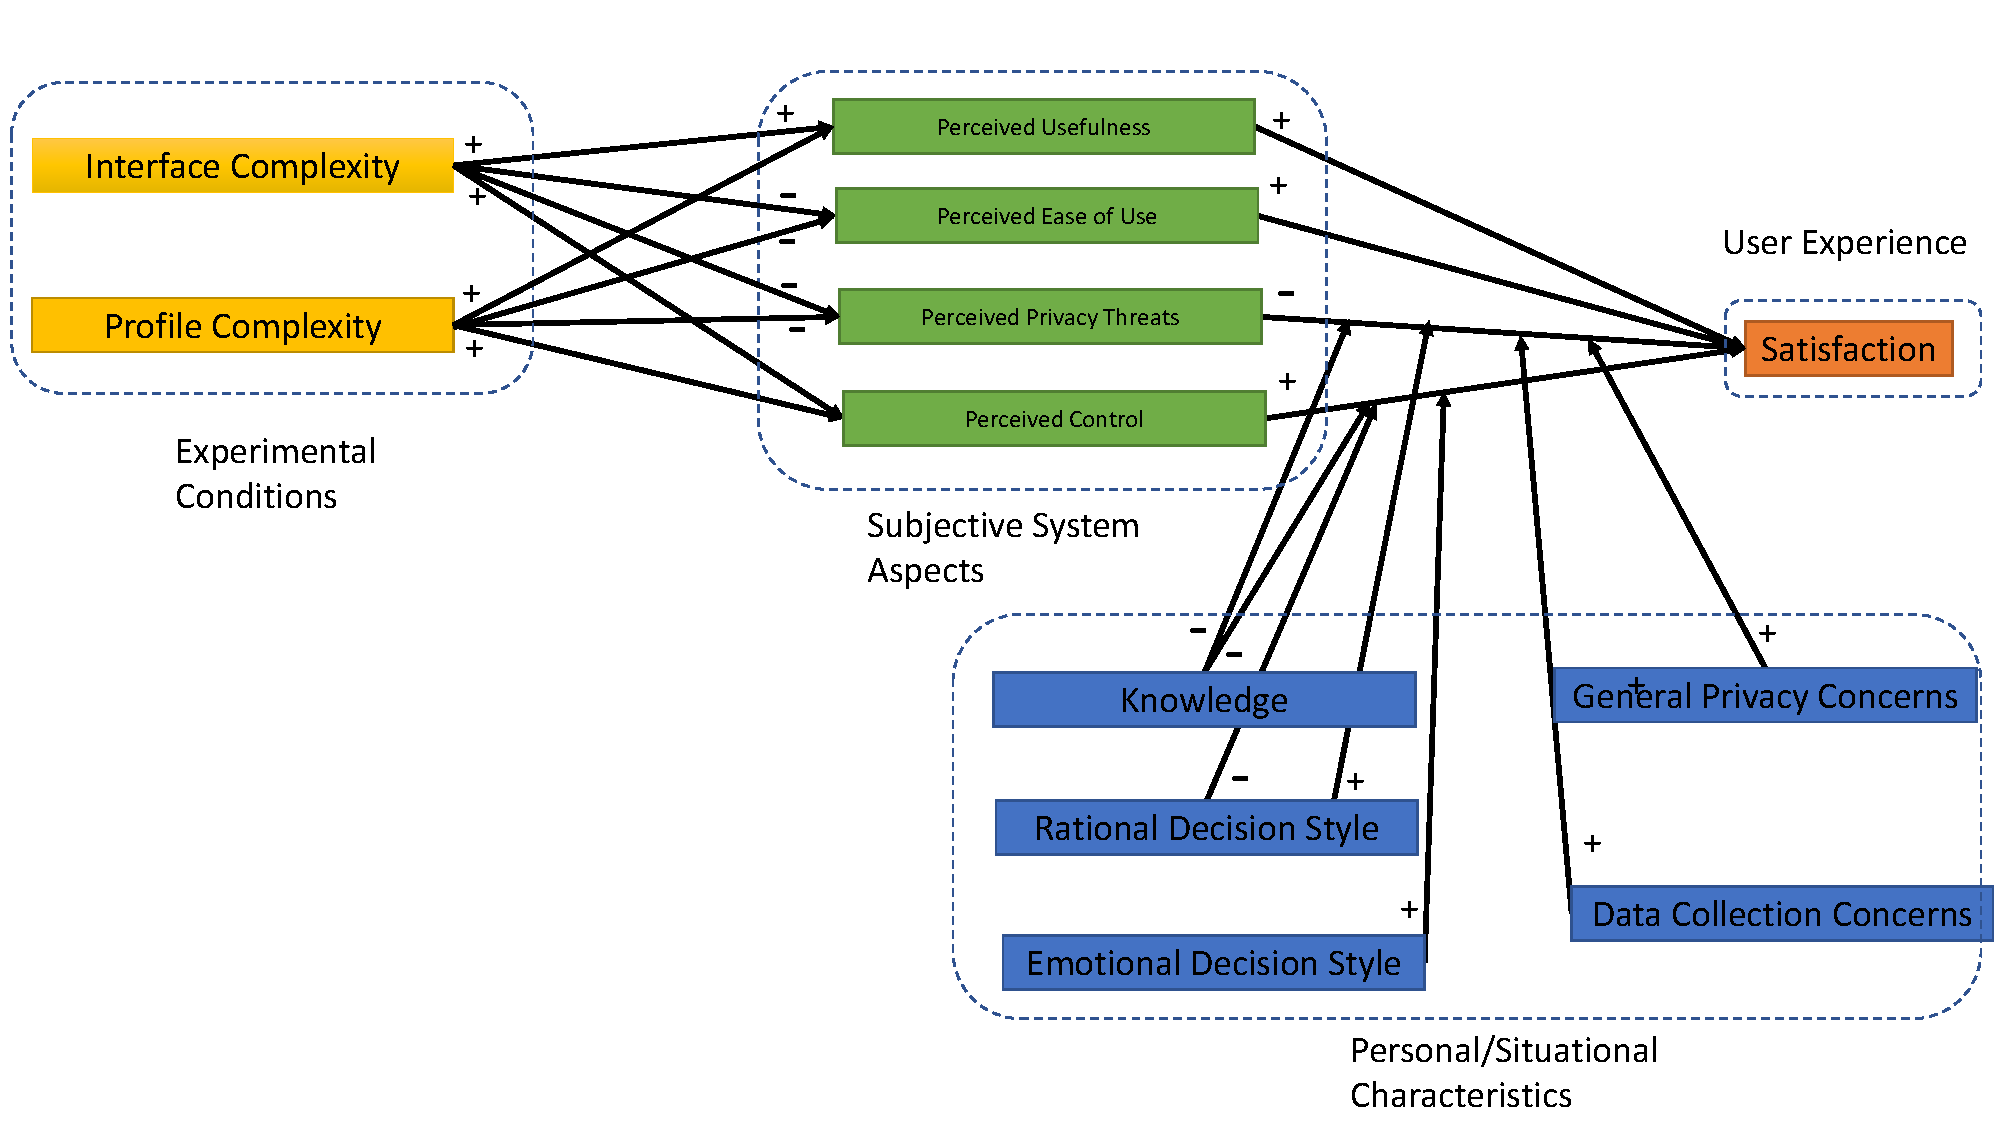
\includegraphics[width=0.9\textwidth]{figures/uimodel.pdf}
%	\caption{Expected Model for Proposed User Study}
%	\label{fig:uimodel}
%\end{figure}

As shown Figure~\ref{fig:uimodel}, we expect `General Privacy Concerns', `Data Collection Concerns', and 'Knowledge' all have a positive effect on the `Perceived Privacy Threats', which consequently has a negative effect on the `Trust' and `Satisfaction'. The mediation effect of `Trust' on `Satisfaction' will also be investigated. The effect of user's decision style is also interesting to us since different style of decision making may have effect on `Perceived Control' or `Perceived Privacy Threats', which will then affect user's `Trust' and `Satisfaction'. `Interface Complexity' is expected to have a positive effect on`Perceived Interface Complexity`, `Perceived Profile Setting Match', `Perceived Control', and `Perceived Ease of Use', which will have a positive effect on `Trust' and `Satisfaction'. `Profile Consevativeness' is expected to have a negative effect on `Perceived Privacy Threats' and a positive effect on `Perceived Control', which will then have a positive effect on both `Trust' and `Satisfaction'.

After the user study is finished, We will use statistics to analysis the effect of the independent variables on the subjective system aspects, and further mediation effect on the user experience. We also wonder how the personal characteristics ans situational characteristics affect the user experience. Finally, we will apply machine learning techniques to uncover deep insights of the results.